\documentclass[a3paper,14pt]{extarticle}
\usepackage{extsizes}
\usepackage{cmap}
\usepackage[utf8]{inputenc}
\usepackage[T2A]{fontenc}
\usepackage[english,russian]{babel} 
\usepackage[left=15mm, top=25mm, right=15mm, bottom=30mm, nohead, nofoot]{geometry}
\usepackage{graphicx}  % изобржаения
\usepackage{xcolor} % определение цветов
\usepackage{nicefrac} % красивые дроби
\usepackage{cancel} % сокращение
\usepackage{amsmath,amsfonts,amssymb} % математический пакет
\usepackage{fancybox,fancyhdr} % хедер и футер
\usepackage{hyperref}  % гиперссылки
\usepackage{tikz} % графика
\pagestyle{fancy}
\fancyhf{}
\fancyhead[L]{Математический анализ}
\fancyhead[R]{Овчинников Павел}
\fancyfoot[C]{\thepage}
\setcounter{page}{1}
\headsep=10mm
\footskip=15mm

\definecolor{urlcolor}{HTML}{3454D1}
\definecolor{linkcolor}{HTML}{3454D1}
\hypersetup{pdfstartview=FitH, linkcolor=linkcolor,urlcolor=urlcolor, colorlinks=true}

\newlength{\tempheight}
\newcommand{\Let}{
\mathbin{\text{\settoheight{\tempheight}{\mathstrut}\raisebox{0.4\pgflinewidth}{
\tikz[baseline=0.5ex,line cap=round,line join=round] \draw (0,0) --++ (0.3em,0) --++ (0,2.3ex) --++ (-0.3em,0);
}}}}
\newcommand\NB{\textbf{N\kern-0.32em\textcolor{red}{B}}}
\newcommand*\circled[1]{\tikz[baseline=(char.base)]{
            \node[shape=circle,draw,inner sep=2pt] (char) {#1};}}
\newcommand*\squared[1]{\tikz[baseline=(char.base)]{
            \node[shape=rectangle,draw,inner sep=4pt] (char) {#1};}}
\newcommand{\at}{\biggr\rvert}

\begin{document}
\section*{\centering Задание №1}
1. Область $D$ ограничена функциями $y = \sqrt{x+2}$, $y = \nicefrac{x^2}{2}$, $y = -x$. Получаем следующий схематический рисунок, на котором эта область выделена цветом и буквой:
\begin{figure}[h]
    \centering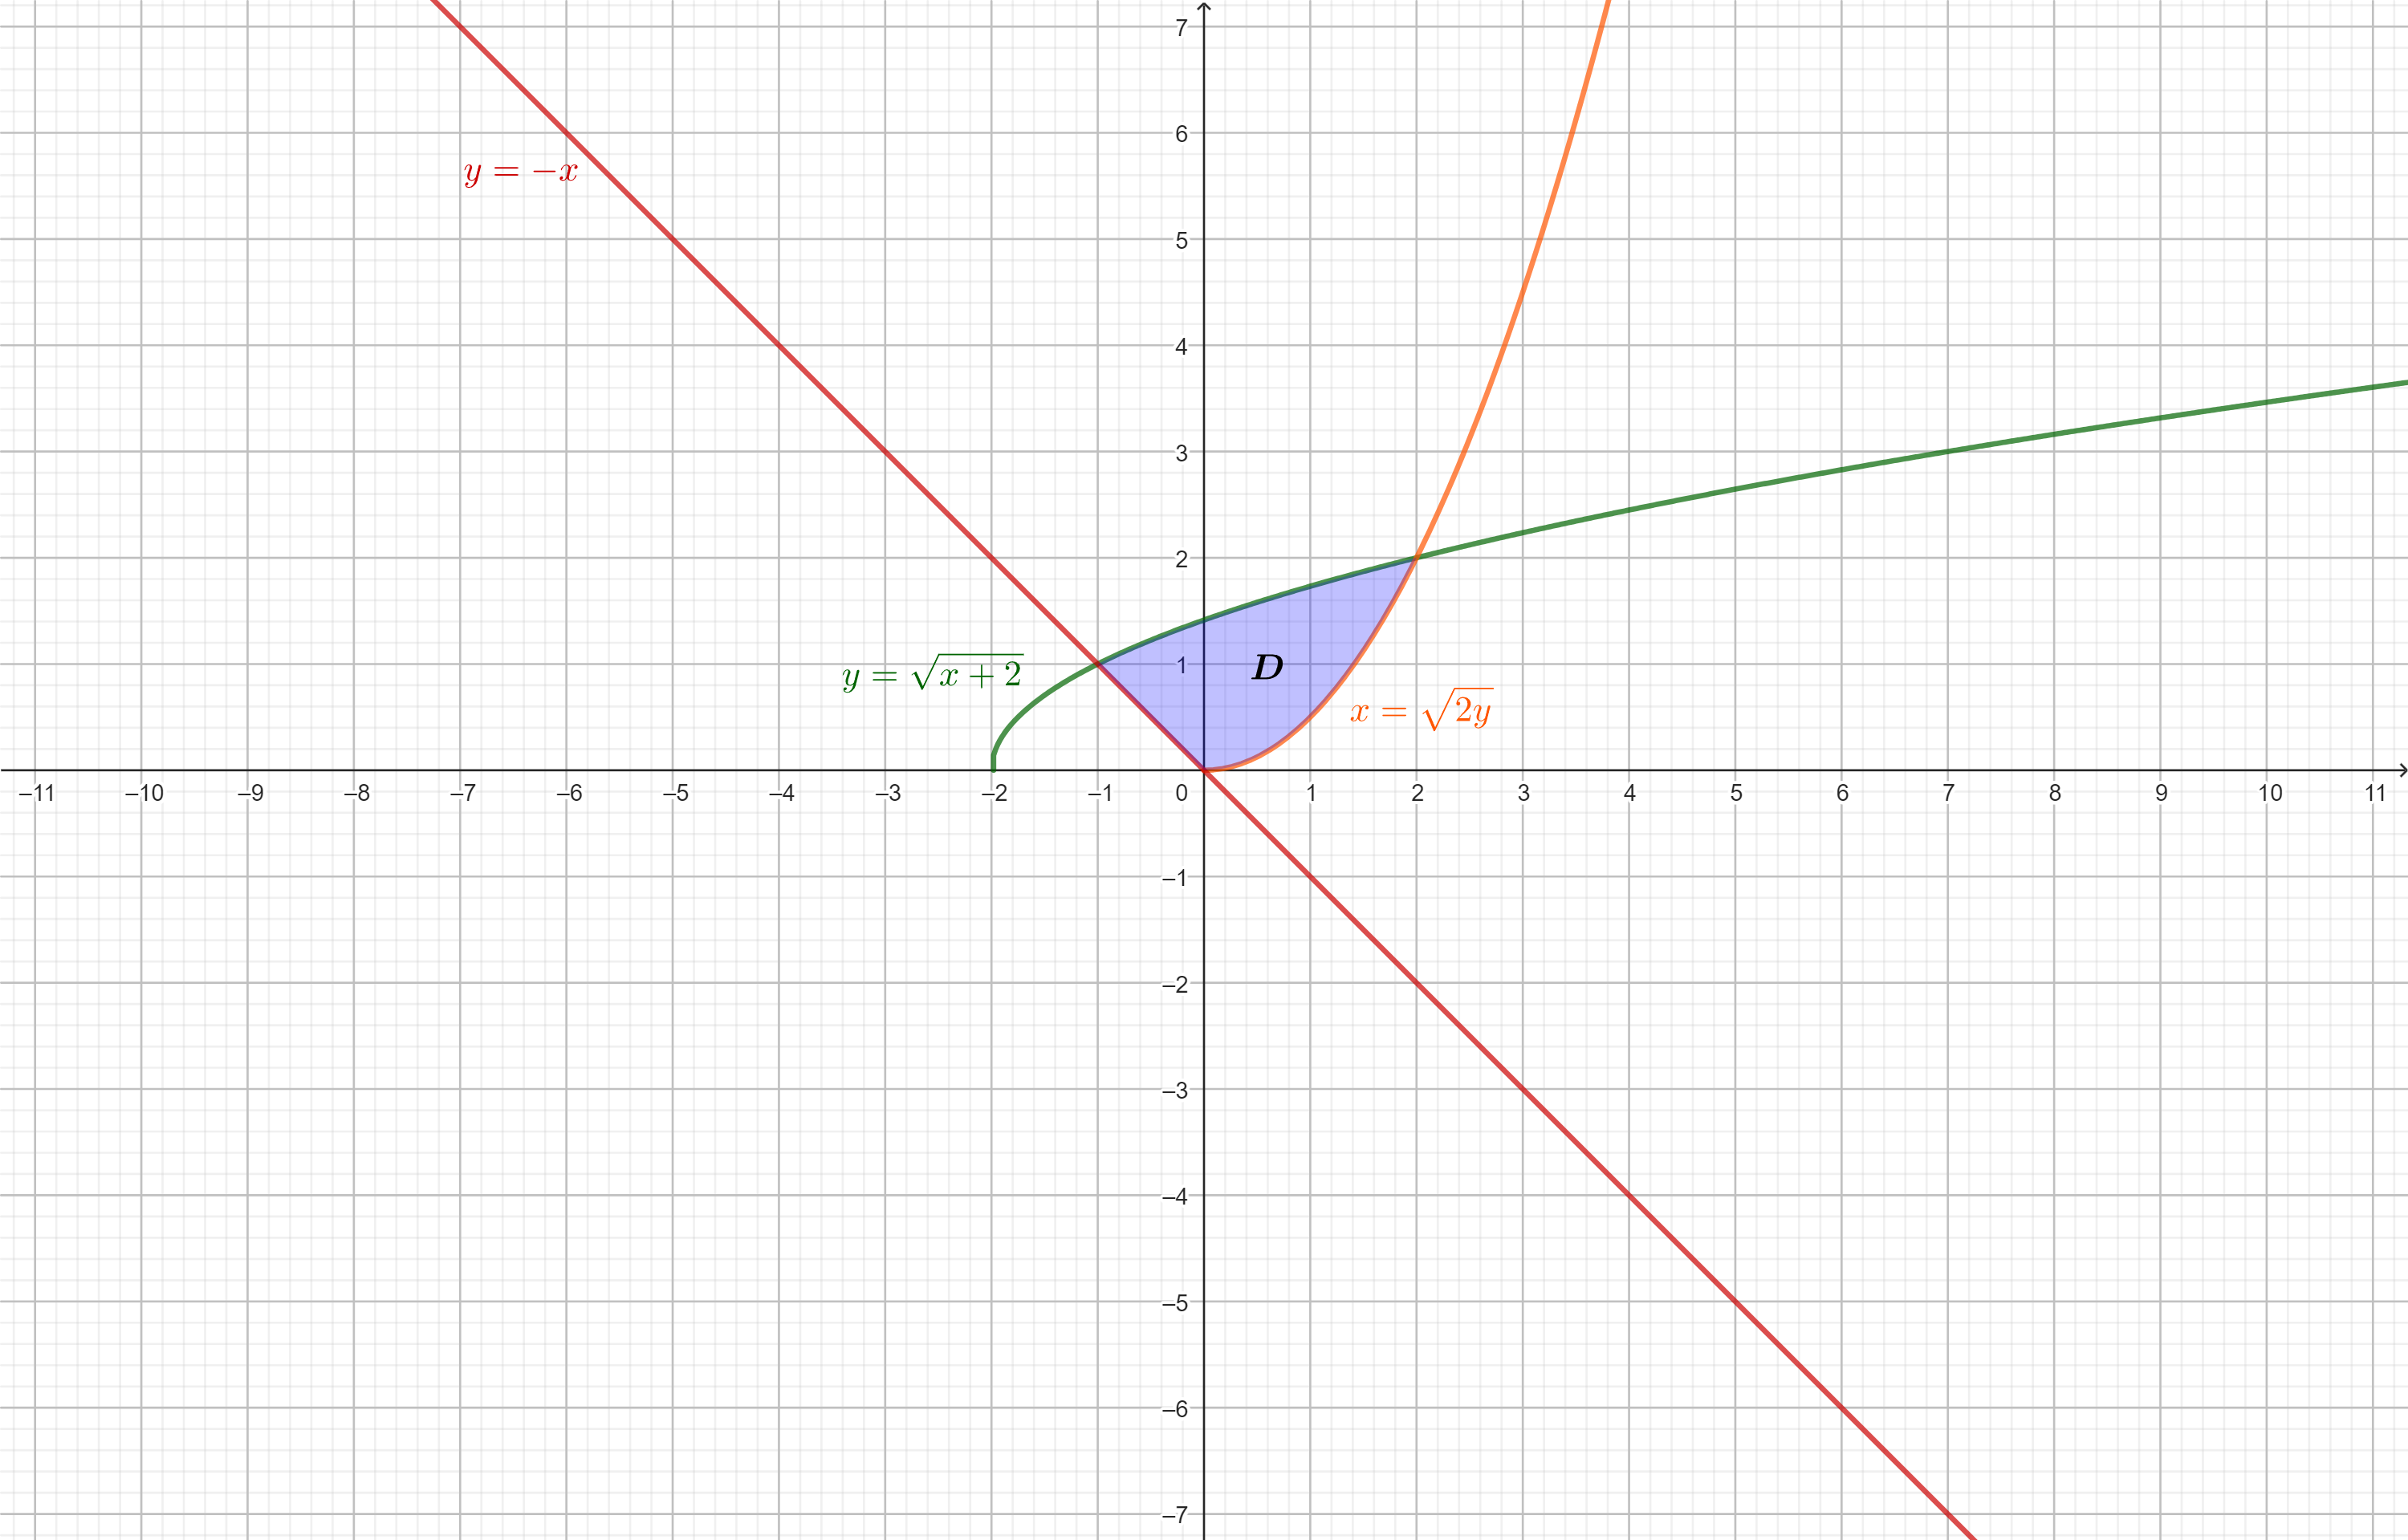
\includegraphics[width=0.5\textwidth]{1.png}
\end{figure} \,\\[1em]
2. Разобъём область на две прямой $x = 0$ и получим области $-1 \le x \le 0$ и $0 \le x \le 2$, а по $y$-координате будем брать интеграл от функций:
$$S_D = \int\limits_{-1}^0dx\int\limits_{-x}^{\sqrt{x+2}}dy \ + \int\limits_0^2dx\int\limits_{\nicefrac{x^2}{2}}^{\sqrt{x+2}}dy = \int\limits_{-1}^0(\sqrt{x+2} + x)dx +\int\limits_0^2\left(\sqrt{x+2} - \frac{x^2}{2}\right)dx = $$
$$ = \left(\frac{2(x+2)\sqrt{x+2}}{3}+\frac{x^2}{2}\right)\at^0_{-1}+\left(\frac{2(x+2)\sqrt{x+2}}{3}-\frac{x^3}{6}\right)\at^2_0 = \cancel{\frac{4\sqrt{2}}{3}} - \frac{7}{6} + 4 - \cancel{\frac{4\sqrt{2}}{3}} = \squared{$\dfrac{17}{6}$}$$

\section*{\centering Задание №2}
1. Тело $T$ ограничено функциями $z = 4 - 2\sqrt{x^2+y^2}$, $z = \frac{x^2+y^2}{2}-2$, $y = 0$. На все функции наложено ограничение $y \ge 0$. Получаем следующий схематический рисунок, на котором конус --- первая функция, параболоид --- вторая, а плоскость --- третья, и кроме этого, конечно, синим выделено интересующее нас тело, объём которого нам необходимо найти:
\begin{figure}[h]
    \centering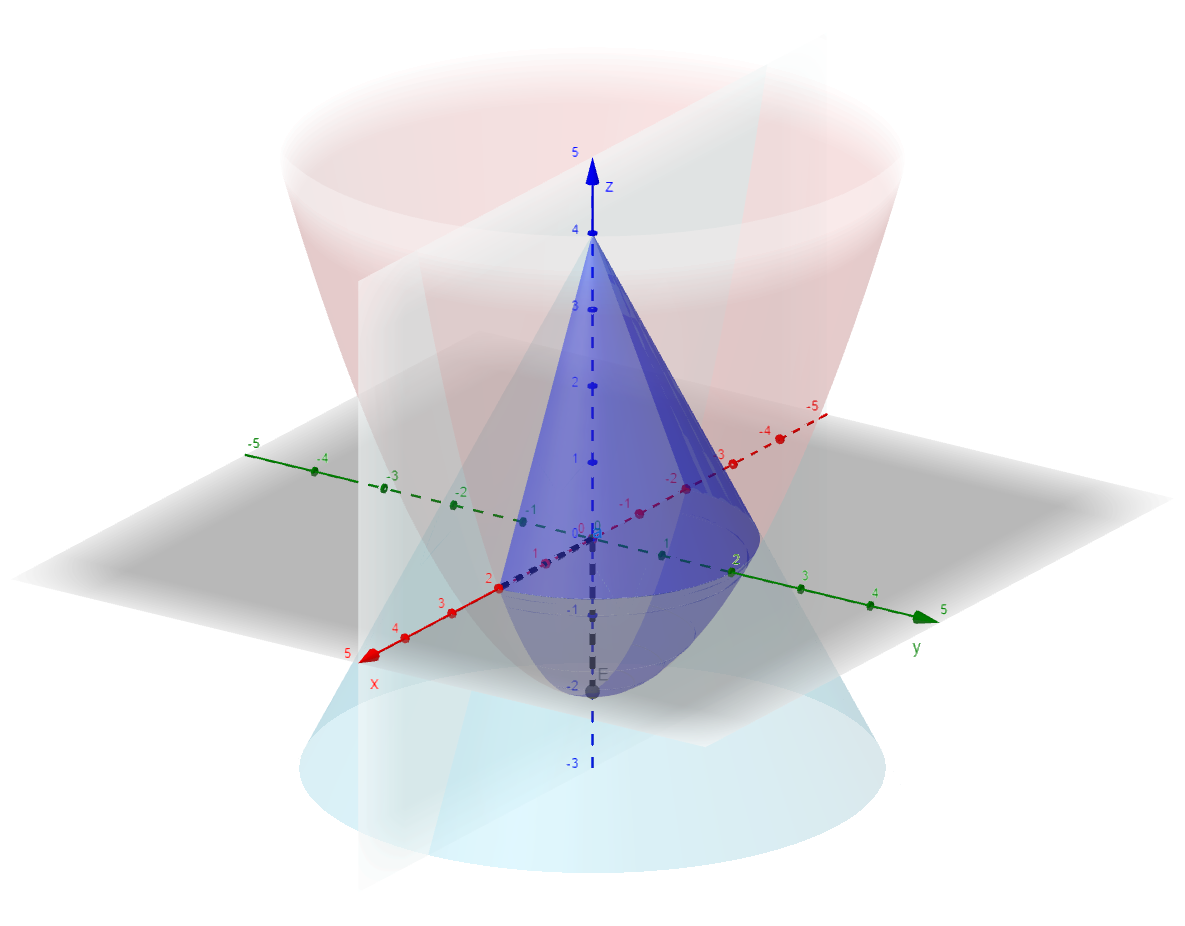
\includegraphics[width=0.66\textwidth]{2.png}
\end{figure}

\pagebreak\noindent 2. Наблюдается тело вращения в рамках развёрнутого угла, поэтому перейдём к цилиндрическим координатам $x=r\cos{\varphi}$, $y=r\sin{\varphi}$. Якобиан перехода будет равен $r$, поэтому интеграл объёма будет выглядеть так: $V = \iiint\limits_T r\,dr\,d\varphi\,dz$. \\
Вот как будут выглядеть после такого перехода уравнения:
\begin{itemize}
    \item конуса --- $z = 4 - 2\sqrt{r^2\cos^2{\varphi}+r^2\sin^2{\varphi}} = 4 - 2r$
    \item параболоида --- $z = \frac{r^2\cos^2{\varphi}+r^2\sin^2{\varphi}}{2}-2=\frac{r^2}{2}-2$
    \item неравенство $y \ge 0$ даст нам $r\sin{\varphi} \ge 0 \Rightarrow \sin{\varphi} \ge 0 \Rightarrow 0 \le \varphi \le \pi$
\end{itemize}
Найдём линию пересечения параболоида и конуса:
$$\begin{cases}
    z = 4 - 2r \\
    z = \frac{r^2}{2}-2 \\
    r \ge 0
\end{cases} \Rightarrow \begin{cases}
    z = 4 - 2r \\
    4 - 2r = \frac{r^2}{2}-2 \\
    r \ge 0
\end{cases} \Rightarrow \begin{cases}
    r = 2 \\
    z = 0
\end{cases}$$
Итак, нам известны пределы $\varphi$, пределы $r$ и для интегрирования мы выбираем две функции, образующие тело вращения, т.е. $\frac{r^2}{2}-2\le z \le 4-2r$. Вычислим интеграл, чтобы найти объём:
$$V = \int\limits_0^\pi d\varphi\int\limits_0^2 r\,dr\int\limits_{\frac{r^2}{2}-2}^{4-2r}dz = \int\limits_0^\pi d\varphi\int\limits_0^2 \left(-\frac{r^3}{2}-2r^2+6r\right)dr = \int\limits_0^\pi \left(-\frac{r^4}{8}-\frac{2r^3}{3}+3r^2\right)\at_0^2d\varphi = \int\limits_0^\pi \frac{14}{3}d\varphi = \squared{$\dfrac{14\pi}{3}$}$$

\section*{\centering Задание №3}
a) Для кривой, заданой уравнением $y = \ln(x^2-1)$ с $\rho(x,y) = 1, x_1 = 3, x_2=5$ масса $M$ дуги может быть вычислена с помощью криволинейного интеграла первого рода:
$$M = \rho(x, y)\int\limits_{x_1}^{x_2}\sqrt{1+(y')^2}\,dx = \int\limits_3^5\sqrt{1+\left(\left(\ln(x^2-1)\right)'\right)^2} =  \int\limits_3^5\sqrt{1+\frac{4x^2}{x^4-2x^2+1}} = \left(x + \ln\left|\frac{x-1}{x+1}\right|\right)\at_3^5 = $$
$$ = 2 + \ln\frac{2}{3} - \ln\frac{1}{2} = \squared{$2 + \ln\dfrac{4}{3}$}$$\,\\[1em]
\hypertarget{from4th}{б)} \label{as} Для кривой, заданной параметрическим способом $x=e^t;\ y=e^{-t}$ с плотностью вещества $\rho(x, y) = \frac{3x^2}{y^3}$, массу её дуги в значениях $t_1 = \frac{1}{4}\ln8, t_2=\frac{1}{4}\ln24$ можно вычислить с помощью всё того же криволинейного интеграла первого рода, но т.к. $x' \ne 1$, то:
$$M =  \int\limits_{t_1}^{t_2}\rho(x, y)\sqrt{(x')^2+(y')^2}\,dt = \int\limits_{\nicefrac{1}{4}\ln8}^{\nicefrac{1}{4}\ln24}\frac{3e^{2t}}{e^{-3t}}\sqrt{e^{2t}-e^{-2t}}\,dt = \int\limits_{\nicefrac{1}{4}\ln8}^{\nicefrac{1}{4}\ln24}3\sqrt{e^{12t}-e^{8t}}\,dt = \frac{1}{2}\left((e^{4t}-1)\sqrt{e^{4t}-1}\right)\at_{\nicefrac{1}{4}\ln8}^{\nicefrac{1}{4}\ln24} = $$
$$= \frac{1}{2}\left((e^{\ln{24}}-1)\sqrt{e^{\ln{24}}-1} - (e^{\ln{8}}-1)\sqrt{e^{\ln{8}}-1}\right) = \frac{1}{2}\left( 23\sqrt{23} - 7\sqrt{7}\right) = \squared{$\dfrac{23\sqrt{23}-7\sqrt{7}}{2}$}$$

\section*{\centering Задание №4}
Задание не сильно отличается от \hyperlink{from4th}{п. \textbf{б}} предыдущего задания. Для материальной кривой в пространстве мы всё так же подставляем в функцию плотности вещества каждое из уравнений, а под корнем берутся квадраты производных уже трёх функций:
$$M = \int\limits_{t_1}^{t_2}\rho(x, y, z)\sqrt{(x')^2+(y')^2+(z')^2}\,dt = \int\limits_{\nicefrac{1}{\sqrt{3}}}^{\sqrt{3}}\frac{1}{7(t^2+1)}\sqrt{(3\sqrt{7}t)^2}\,dt = \frac{3\sqrt{7}}{7}\int\limits_{\nicefrac{1}{\sqrt{3}}}^{\sqrt{3}}\frac{t}{t^2+1} = \frac{3\sqrt{7}}{14}\ln{(t^2+1)}\at_{\nicefrac{1}{\sqrt{3}}}^{\sqrt{3}} =$$
$$ = \frac{3\sqrt{7}}{14}\left( \ln{4} - \ln{\frac{4}{3}}\right) = \squared{$\dfrac{3\sqrt{7}\ln{3}}{14}$}$$ \pagebreak\noindent

\section*{\centering Задание №5}
Нам дано векторное поле $\vec{a} = (3y+z)\vec{j}-3(x+y)\vec{k}$ и плоскость $\sigma\colon 3x-3y+z=-3$. Представлю в декартовом пространстве векторное поле, чтобы не возвращаться к его визуализации далее в пунктах задания (плоскость визуализируем в \hyperlink{fromabove}{п. \textbf{1}}):
\begin{figure}[h]
    \centering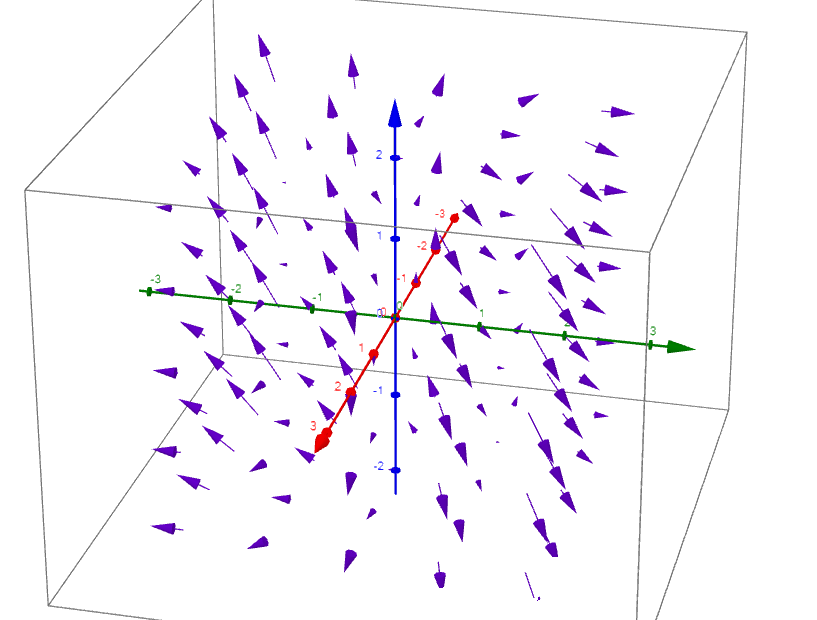
\includegraphics[width=0.5\textwidth]{5.0.png}
\end{figure} \,\\[1em]
\hypertarget{fromabove}{1.} Чтобы найти поток $Q$ поля $\vec{a}$ через поверхность $S$, образованной $\triangle KLM$, нам понадобится в первую очередь скромная визуализация, а затем поверхностный интеграл первого рода $\iint\limits_S\vec{a}\cdot\vec{n}\,dS$, где $\vec{n}$ --- нормаль плоскости $\sigma$, направленная из начала координат. И вот как это всё выглядит на рисунке:
\begin{figure}[h]
    \centering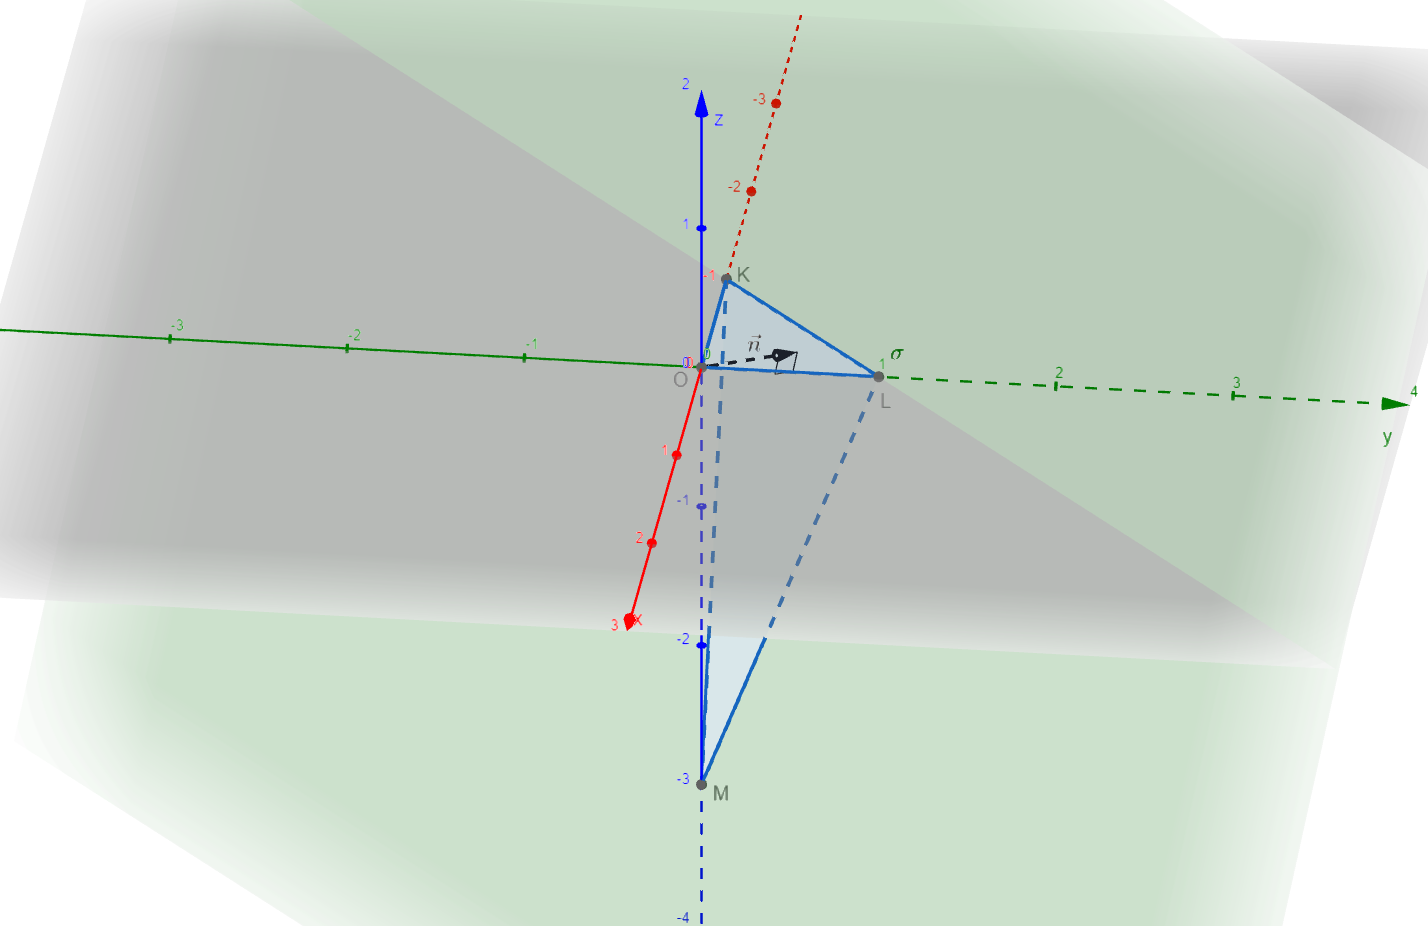
\includegraphics[width=0.5\textwidth]{5.1.png}
\end{figure} \,\\[1em]
Плоскость $\sigma$ пересекает ось $Oz$ в точке $M$, ось $Oy$ --- в точке $L$ и ось $Ox$ --- в точке $K$. И теперь необходимо разобраться в интеграле. $\vec{a}$ выражается своими составляющими $a_y = 3y + z$ и $a_z = -3(x+y)$, а $\vec{n}$ можно представить как вектор, отклонённый на углы $\alpha, \beta, \gamma$ от осей $Ox$, $Oy$ и $Oz$ соответственно. И тогда скалярное произведение $\vec{a}\cdot\vec{n} = a_y\cos{\beta} + a_z\cos{\gamma}$ (произведение $a_x\cos{\alpha}$ отсутствует, т.к. $a_x = 0$). \\[1em]
Мы будем проецировать всё на плоскость $Oxy$, поэтому нам понадобятся функции $p(x,y) = \frac{\partial z}{\partial x}$ и $q(x,y) = \frac{\partial z}{\partial y}$ (здесь $z$ --- уравнение плоскости $\sigma$, решённое относительно этой переменной), благодаря которым мы сможем ввести функцию $D(x,y) = \sqrt{1+p^2(x,y)+q^2(x,y)}$. И с этой функцией дифференциал $dS$ можно представить как $dS = D(x,y)\,dxdy$, а $\cos{\beta} = \frac{-q(x,y)}{\pm D(x,y)}$ и $\cos{\gamma} = \frac{1}{\pm D(x,y)}$. Знак $\pm$ перед $D(x,y)$ выбирается в зависимости от того, какой угол образует нормаль с осью $Oz$ --- в формулы ставится $+$, если он острый, и в нашем случае ставится $-$.\\[1em]
Найдём $p(x,y)$, $q(x,y)$ и $D(x,y)$:
$$p(x,y) = \frac{\partial z}{\partial x} = (3y-3x-3)'_x = -3\qquad q(x,y) = \frac{\partial z}{\partial y} = (3y-3x-3)'_y = 3$$
$$D(x, y) = \sqrt{1+9+9} = \sqrt{19}$$
Преобразуем в соответствии с полученной информацией наш поверхностный интеграл в интеграл по площади $\triangle OKL$ --- спроецированный $\triangle KLM$ на плоскость $Oxy$, заменив на последнем шаге $z$ на уравнение плоскости $\sigma$, решённое относительно этой переменной: $$\iint\limits_S\vec{a}\cdot\vec{n}\,dS = \iint\limits_S (a_y\cos{\beta} + a_z\cos{\gamma})\,dS = \iint\limits_{OKL} \cancel{D(x,y)}\left( (3y + z)\frac{q(x,y)}{\cancel{D(x,y)}} + \frac{3(x + y)}{\cancel{D(x,y)}} \right)\,dxdy = $$
$$= \iint\limits_{OKL} \left( 3(3y + z) + 3(x + y) \right)\,dxdy = 3\iint\limits_{OKL} \left(x + 4y + z \right)\,dxdy = 3\iint\limits_{OKL} \left( 7y - 2x - 3 \right)\,dxdy$$
Нам остаётся только определить пределы интегрирования. Для этого посмотрим, какая прямая соответствует гипотенузе спроецированного $\triangle OKL$:
\begin{figure}[h]
    \centering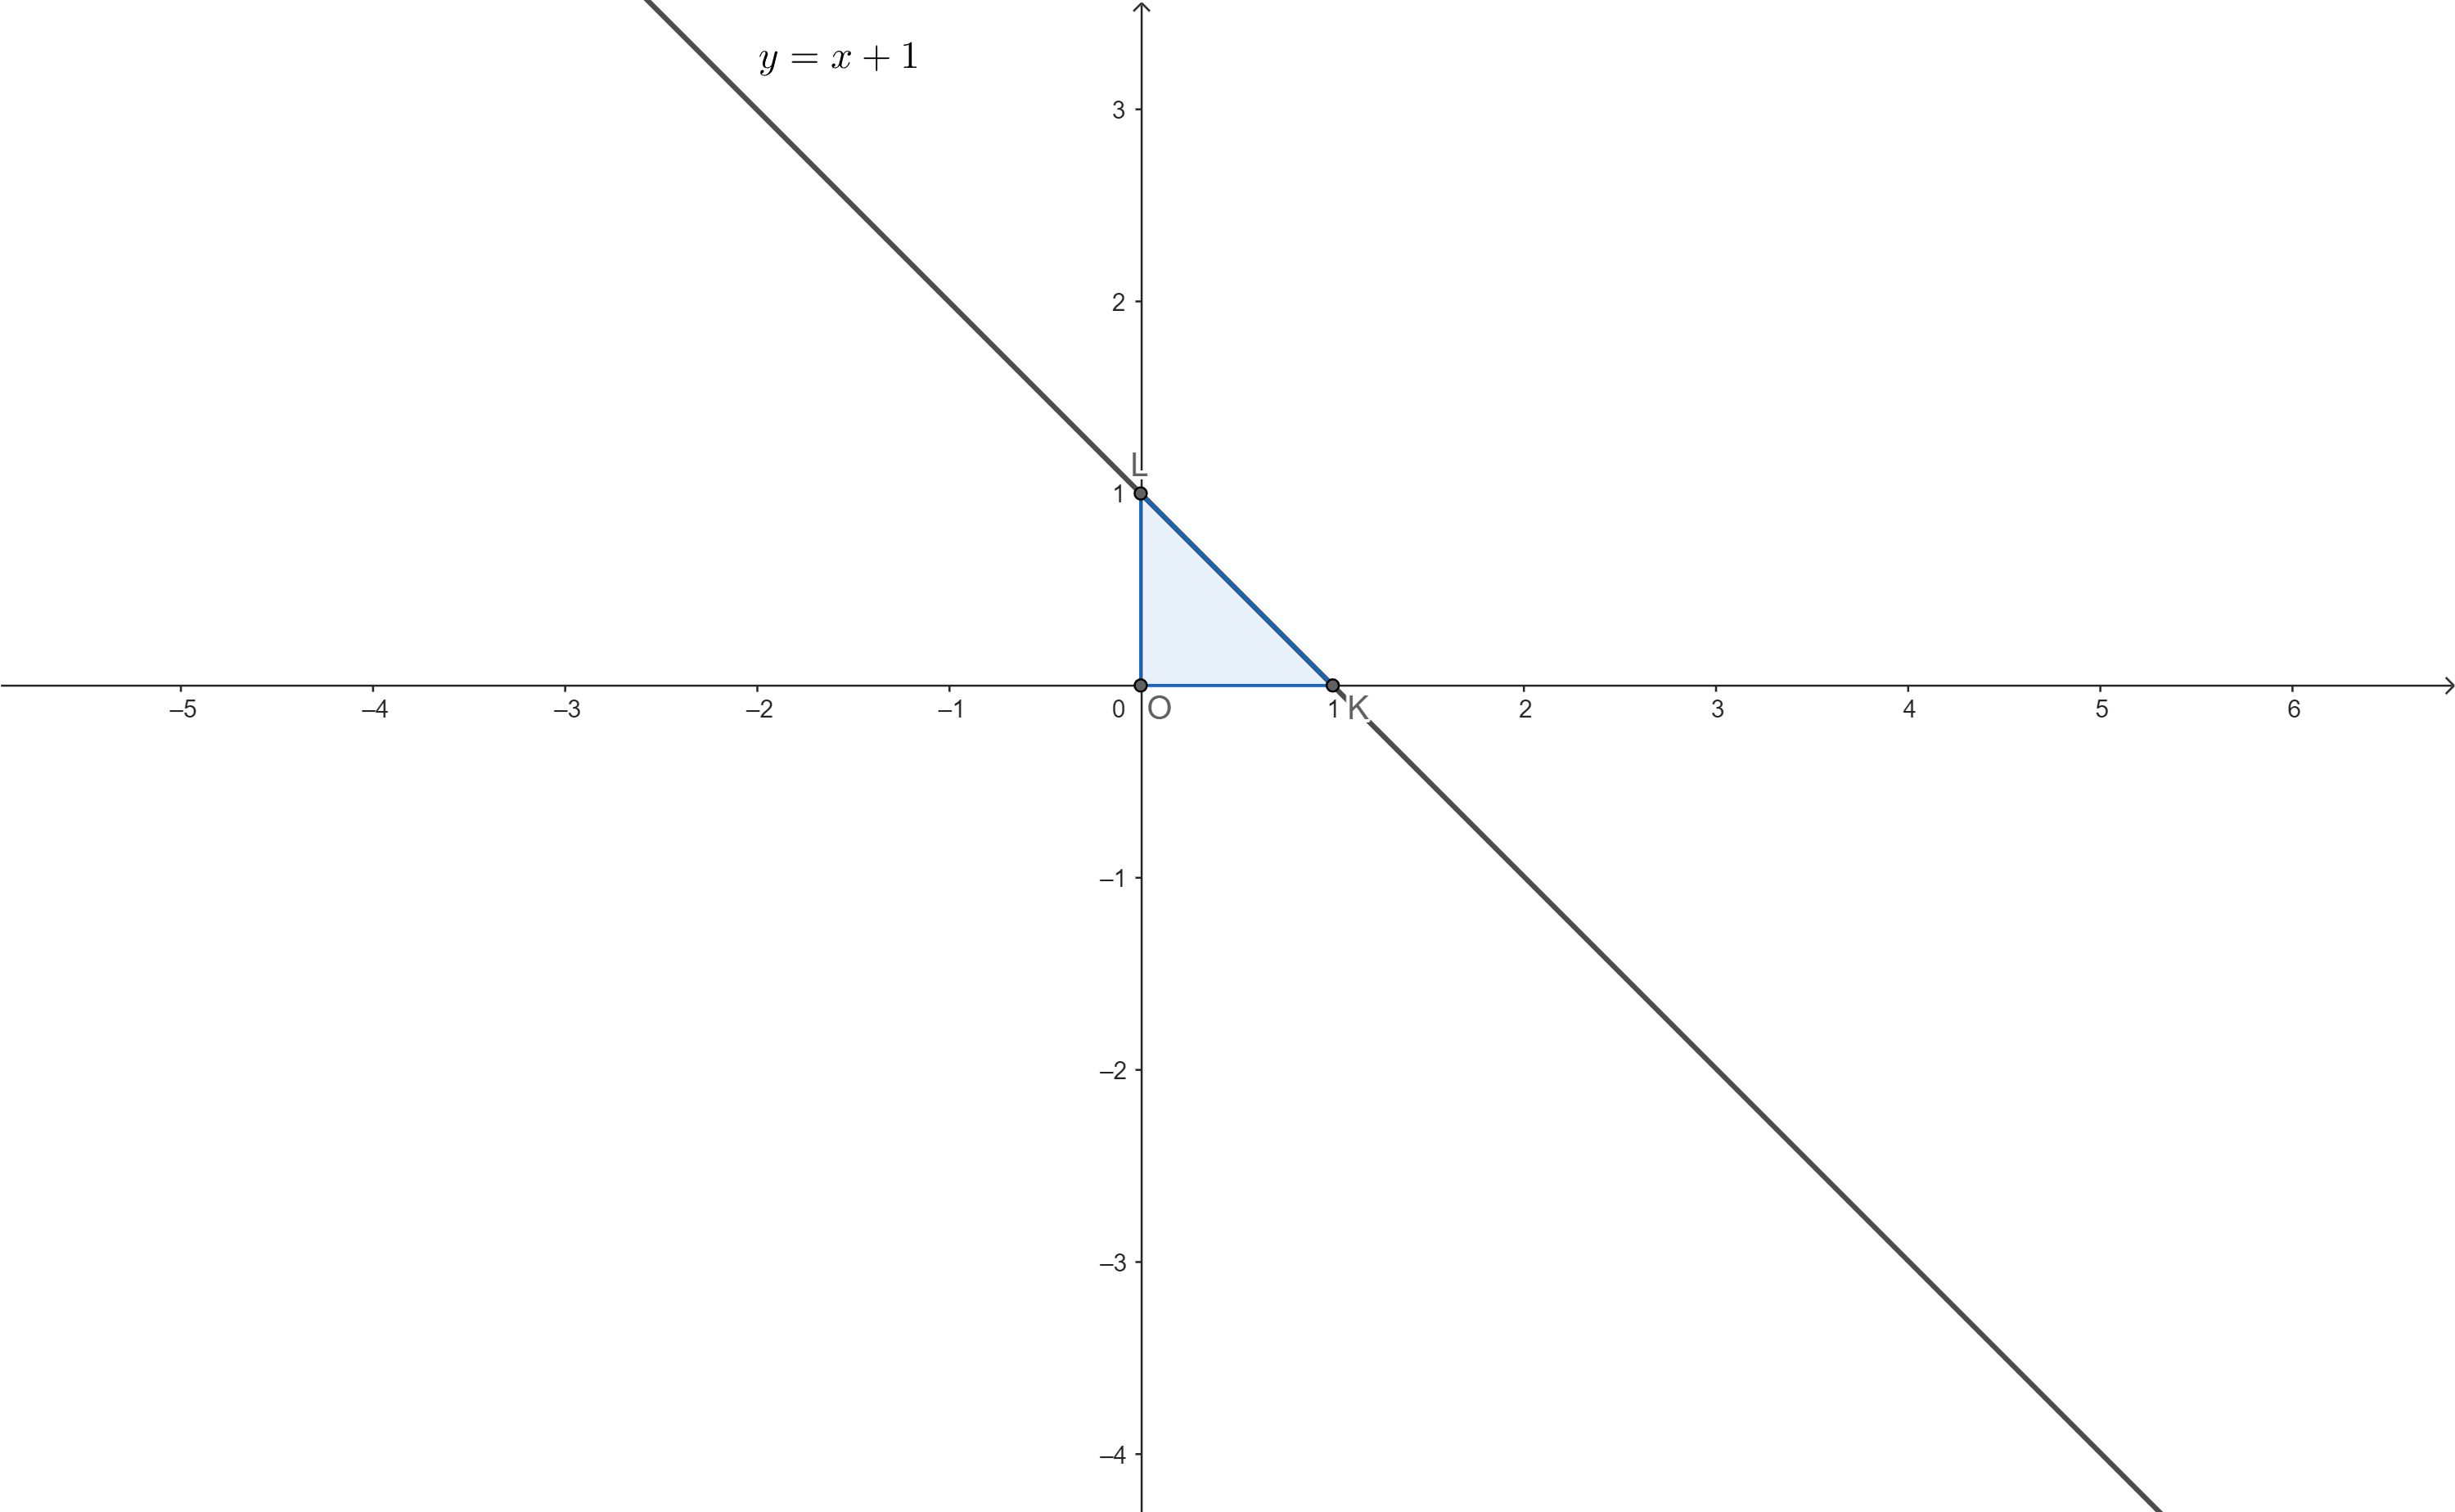
\includegraphics[width=0.5\textwidth]{5.1 triangle.png}
\end{figure} \,\\[1em]
По оси $Ox$ интегрируем от $-1$ до $0$ и по оси $Oy$ --- от $0$ до $x+1$:
$$3\int\limits_{-1}^0 dx \int\limits_0^{x+1} \left( 7y - 2x - 3 \right)\,dy = 3\int\limits_{-1}^0 dx\left( \frac{7y^2}{2} - 2xy - 3y \right)\at_0^{x+1} = 3\int\limits_{-1}^0 \left( \frac{3x^2}{2}+2x+\frac{1}{2} \right)\,dx = -3\left( -\frac{1}{2}+1-\frac{1}{2} \right) = \squared{$0$}$$\\[2em]
2. Формула Остроградского-Гаусса для вычисления потока $Q$ векторного поля $\vec{a}$ через замкнутую поверхность $T$ выглядит так: $Q = \iiint\limits_T\text{div}\vec{a}\,dv$. Посчитаем дивергенцию: $$\text{div}\vec{a} = \frac{\partial a_x}{\partial x} + \frac{\partial a_y}{\partial y} + \frac{\partial a_z}{\partial z} = \frac{\partial 0}{\partial x} + \frac{\partial (3y+z)}{\partial y} + \frac{\partial (-3(x+y))}{\partial z} = 3$$
Теперь интеграл принимает вид $Q = 3\iiint\limits_T dv = 3V_T$. Объём тетраэдра вычислим по формуле: $$V_T = \frac{1}{6}\cdot OM\cdot OK\cdot OL = \frac{1}{6}\cdot3\cdot1\cdot1 = \frac{1}{2} \quad \Rightarrow \quad Q = 3\cdot\frac{1}{2} = \squared{$1.5$}$$\\[2em]
3. Для вычисления циркуляции $C$ векторного поля $\vec{a}$ по контуру $l = KLMK$ необходим криволинейный интеграл второго рода:
$$C = \int\limits_{l}\vec{a}\cdot d\vec{r}= \int\limits_{l}a_x\,dx + a_y\,dy + a_z\,dz = \int\limits_{l}(3y + z)\,dy - 3(x + y)\,dz$$

\pagebreak\noindent Думаю, тут необходимо продемонстрировать контур, чтобы было понятно, каким образом нужно считать:
\begin{figure}[h]
    \centering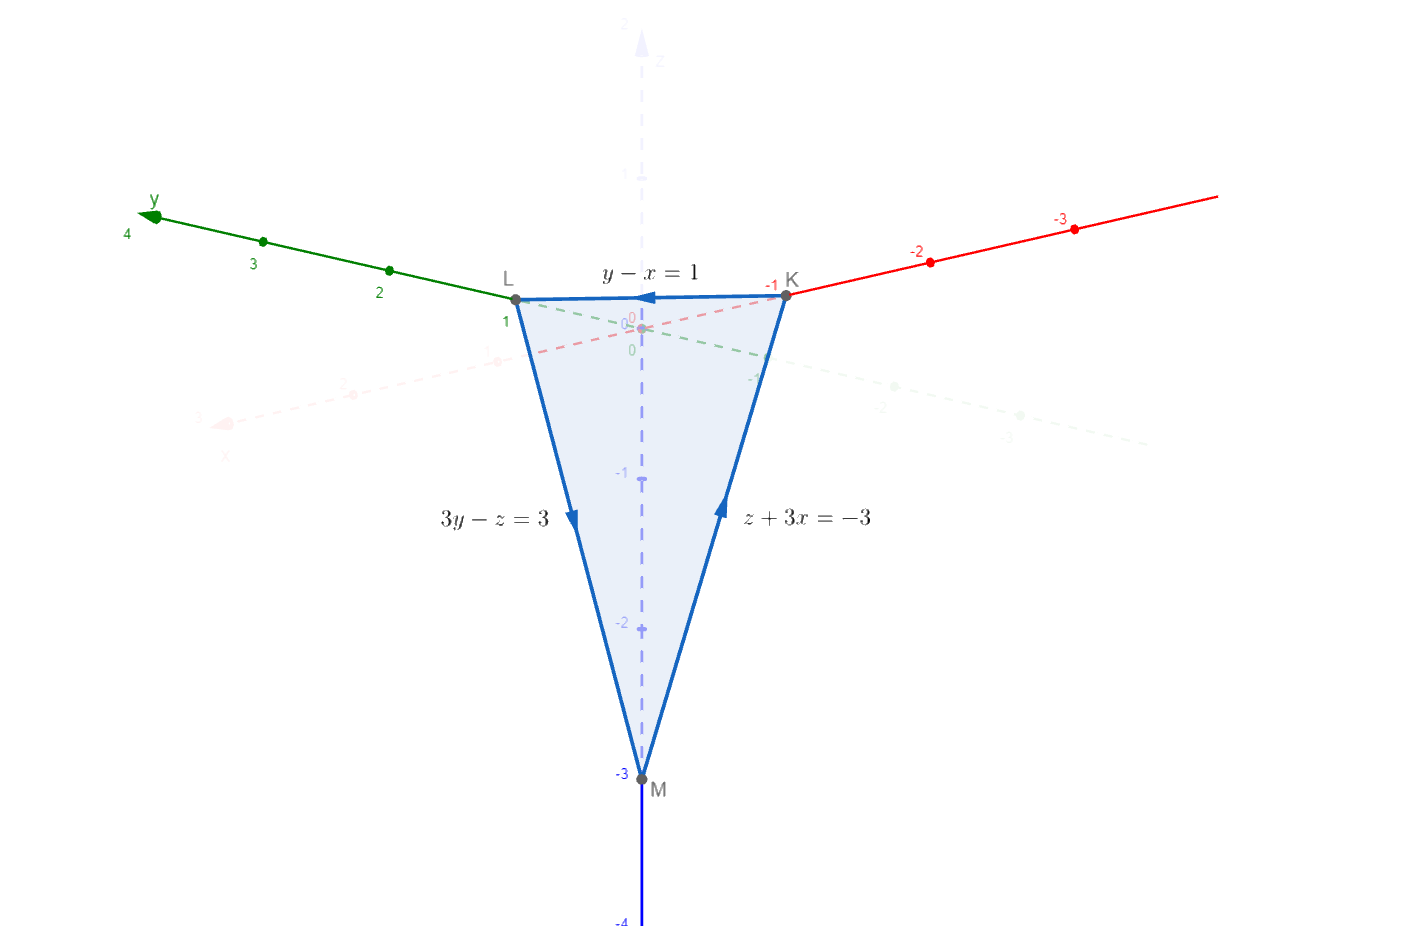
\includegraphics[width=0.5\textwidth]{5.3.png}
\end{figure} \,\\[1em]
Теперь с таким интегралом пройдёмся по каждой составляющей контура, чтобы найти сумму $C = I_{KL} + I_{LM} + I_{MK}$:
\begin{enumerate}
    \item $I_{KL}$: $\begin{cases}
        z = 0 \\ y-x = 1
    \end{cases} \Rightarrow \begin{cases}
        dz = 0 \\ z = 0
    \end{cases}$ c пределами интегрирования $0 \le y \le 1$ подставим в интеграл $I_{KL} = \int\limits_0^1 3y\,dy = \frac{3}{2}$.
    \item $I_{LM}$: $\begin{cases}
        x = 0 \\ z = 3y - 3
    \end{cases} \Rightarrow \begin{cases}
        x = 0 \\ dz = 3dy \\ z = 3y - 3
    \end{cases}$ с пределами $1 \ge y \ge 0$ подставим в интеграл $I_{LM} = \int\limits_1^0 (-3y-3)\,dy = \frac{9}{2}$.
    \item $I_{MK}$: $\begin{cases}
        y = 0 \\ z = -3x - 3
    \end{cases} \Rightarrow \begin{cases}
        y = 0 \\ dy = 0 \\ dz = -3dx
    \end{cases}$ с пределами $0 \ge x \ge -1$ подставим в интеграл $I_{MK} = \int\limits_0^{-1} 9x\,dx = \frac{9}{2}$.
\end{enumerate}
Общей циркуляцией $C$ поля будет сумма $C = I_{KL} + I_{LM} + I_{MK} = \frac{3}{2} + \frac{9}{2} + \frac{9}{2} = \squared{$10.5$}$.

\section*{\centering Задание №6}
Дано векторное поле $\vec{a} = 2x(y+z)\vec{i} + (x^2-y^2)\vec{j} + (x^2-z^2+3)\vec{k}$.\\[1em]
1. Проверим, является ли векторное поле соленоидальным --- то есть равна ли дивергенция поля нулю:
$$\text{div}\vec{a} = \frac{\partial (2x(y+z))}{\partial x} + \frac{\partial (x^2-y^2)}{\partial y} + \frac{\partial (x^2-z^2+3)}{\partial z} = \cancel{2y} + \bcancel{2z} - \cancel{2y} - \bcancel{2z} = 0$$
\squared{Поле соленоидальное.}\\[0.5em]
Проверим, является ли векторное поле потенциальным --- для этого необходимо выяснить, равен ли ротор поля нулю:
$$\text{rot}\vec{a} = \begin{vmatrix}
    \vec{i} & \vec{j} & \vec{k} \\
    \dfrac{\partial}{\partial x} & \dfrac{\partial}{\partial y} & \dfrac{\partial}{\partial z} \\
    2x(y + z) & x^2-y^2 & x^2-z^2+3
\end{vmatrix} = \left( \frac{\partial(x^2-z^2+3)}{\partial y} - \frac{\partial(x^2-y^2)}{\partial z} \right)\vec{i} + \left( \frac{\partial(2x(y+z))}{\partial z} - \frac{\partial(x^2-z^2 + 3)}{\partial x} \right)\vec{j} + $$
$$+ \left( \frac{\partial(x^2-y^2)}{\partial x} - \frac{\partial(2x(y+z))}{\partial y} \right)\vec{k} = 0\vec{i} + (2x - 2x)\vec{j} + (2x - 2x)\vec{k} = 0$$
Ротор при любых значениях переменных равен нулю, поэтому \squared{поле потенциальное.}

\pagebreak\noindent 2. Т.к. поле потенциально, нам необходимо найти его потенциал --- такое скалярное поле $U$, что его градиент будет равен исходному векторному полю, т.е $\vec{a} = \text{grad}\,U$. Дифференциал такого поля при этом равен $dU = a_x\,dx + a_y\,dy + a_z\,dz$. Это значит, что справедливо $U = \int\limits_{M_0}^M dU + C$, где $M_0$ --- начальная точка интегрирования, а $M$ --- конечная.\\[0.5em]
В нашем случае получаем такой интеграл $U = \int\limits_{M_0}^M 2\tilde{x}(\tilde{y}+\tilde{z})\,d\tilde{x} + (\tilde{x}^2-\tilde{y}^2)\,d\tilde{y} + (\tilde{x}^2-\tilde{z}^2+3)\,d\tilde{z}$. Мы начнём с точки $M(0; 0; 0)$ и будем последовательно добавлять $x$, $y$ и $z$ к исходное точке. На рисунке можно подробно рассмотреть ломанную $OABM$, по которой мы будем поэлементно вычислять интегралы и потенциалом станет сумма этих интегралов.
\begin{figure}[h]
    \centering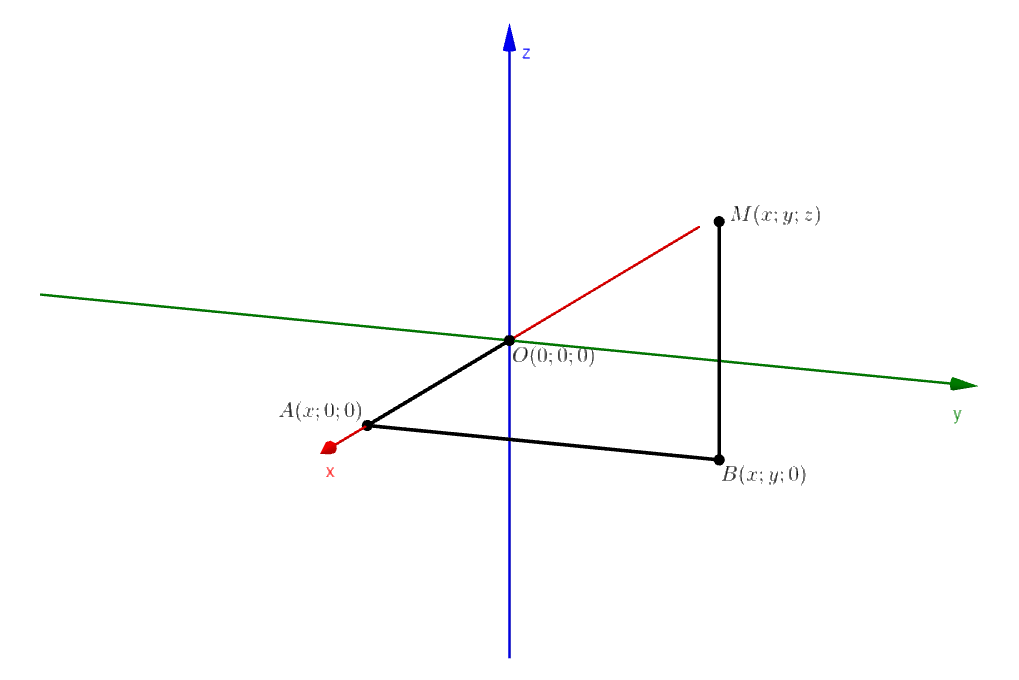
\includegraphics[width=0.4\textwidth]{6.png}
\end{figure} \,\\[1em]
\begin{enumerate}
    \item $I_{OA}$: $\begin{cases}
        \tilde{y} = 0 \\ \tilde{z} = 0
    \end{cases}$, вне зависимости от выбранных пределов получаем $\int 0dx = 0$.
    \item $I_{AB}$: $\begin{cases}
        \tilde{x} = x = \text{const} \\ \tilde{z} = 0
    \end{cases} \Rightarrow \begin{cases}
        d\tilde{x} = 0 \\ d\tilde{z} = 0
    \end{cases}$ c пределами интегрирования $0 \le \tilde{y} \le y$ получаем $\int\limits_0^y (\tilde{x}^2-\tilde{y}^2)\,d\tilde{y} = x^2y - \frac{y^3}{3}$.
    \item $I_{BM}$: $\begin{cases}
        \tilde{x} = x = \text{const} \\ \tilde{y} = y = \text{const}
    \end{cases} \Rightarrow \begin{cases}
        d\tilde{x} = 0 \\ d\tilde{y} = 0
    \end{cases}$ c пределами $0 \le \tilde{z} \le z$ получаем $\int\limits_0^z (\tilde{x}^2-\tilde{z}^2+3)\,d\tilde{z} = x^2z - \frac{z^3}{3}+3z$.
\end{enumerate}
Итак, потенциал векторного поля $\vec{a}$ --- скалярное поле $U = I_{OA} + I_{AB} + I_{BM} + C = \squared{$x^2(y + z) - \frac{y^3}{3} - \frac{z^3}{3} + 3z + C$.}$
\end{document}